\documentclass[a4paper]{article}

%% Language and font encodings
\usepackage[english]{babel}
\usepackage[utf8x]{inputenc}
\usepackage[T1]{fontenc}

%% Sets page since and margins
\usepackage[a4paper,top=3cm,bottom=2cm,left=3cm,right=3cm,marginparwidth=1.75cm]{geometry}

%% Useful packages
\usepackage{amsmath}
\usepackage{graphicx}
\usepackage[colorinlistoftodos]{todonotes}
\usepackage[colorlinks=true, allcolors=blue]{hyperref}
\usepackage{bm}
\usepackage{amsfonts}

% Note the substitute command needs to be enclosed in double brackets
% otherwise the bold font spills out of the command
\newcommand{\vzero}{{\bf 0}}
\newcommand{\vI}{{\bf I}}
\newcommand{\vb}{{\bf b}}
\newcommand{\vd}{{\bf d}}
\newcommand{\vf}{{\bf f}}
\newcommand{\vc}{{\bf c}}
\newcommand{\vp}{{\bf p}}
\newcommand{\vv}{{\bf v}}
\newcommand{\vz}{{\bf z}}
\newcommand{\vn}{{\bf n}}
\newcommand{\vm}{{\bf m}}
\newcommand{\vG}{{\bf G}}
\newcommand{\vQ}{{\bf Q}}
\newcommand{\vM}{{\bf M}}
\newcommand{\vW}{{\bf W}}
\newcommand{\vX}{{\bf X}}
\newcommand{\vPsi}{{\bf \Psi}}
\newcommand{\vSigma}{{\bf \Sigma}}
\newcommand{\vlambda}{{\bf \lambda}}
\newcommand{\vpi}{{\bm \pi}}
\newcommand{\vtheta}{{\bm \theta}}
\newcommand{\valpha}{{\bm{\alpha}}}
\newcommand{\vLambda}{{\bf \Lambda}}
\newcommand{\vA}{{\bf A}}
\newcommand{\E}{\mathbb{E}}



\title{Mutect2 Orientation Artifact Filter}
\author{Takuto Sato}


\begin{document}
\maketitle

\section{Terminology}
Clearly define:
Forward strand
Reverse strand

\section{Intro}
We will first discuss how orientation bias arises during sequencing. To do so we will go over Kap ICE library construction (also known as library prep) and a bit of Illumina sequencing. We will abbreviate and abstract the steps along the way to befit our purpose, which again is to understand how orientation bias arises during sequencing. The sequencing protocol described below is Kapa ICE exome. 

We first take vial full of DNA molecules and shear them into fragments. The resulting fragments of DNA, as depicted in the Figure \ref{fig:oxog}, are called \textit{inserts}. Without loss of generality we assume that the strand shown on top in blue is the \textit{forward} strand; that is, read from 5' end to 3' end, bases in the blue strand map directly to the reference. The strand in orange, conversely, is a \textit{reverse} strand, as it is a reverse complement of the reference when read from 5' to 3' end.

Few years back, folks at GP found that high-power acoustic shearing (as opposed to enzymatic shearing as in Nexome Library Construction) may cause guanine (G) in the insert to oxidize. The oxidized G may base-pair with adenine (A) in addition to the regular cytosine (C). The oxidized G is depicted as a G* with an asterisk in the figures; thus the forward strand at the top of the figure contains an oxidized G near the 5' end.

Next in library prep we add adapters to the double-stranded inserts. In ICE Kapa Exome protocol, we only use one kind of adapter, shown as red and green fragments in Figure \ref{fig:oxog}, and this one type of (double-stranded) adapter attaches to both sides of the insert. To reiterate, the adapters on the left and right side are identical, but, due to directionality of the DNA molecule, they are flipped. We call a DNA insert with adapters attached a \text{library}. To distinguish them from the libraries created in subsequent PCR, we call this insert an \textit{original library}, in the sense that they are not PCR duplicates of the DNA.

Next we denature the original library and run PCR. PCR replicates of the forward strand are shown on the bottom left corner in the figure. Note that during PCR G* in the forward strand base paired with A, which, after another round of PCR, created a third duplicate with a T in place of the original G. PCR replicates the reverse strand, shown in deep orange, faithfully and thus we get only one type of PCR duplicate\footnote{in reality this is unlikely. But since we are talking about an idealized, abstracted world anyway, we are free to suppose that this is the case}. 

Now we pour the libraries on the flowcell, as detailed in Figure \ref{fig:flowcell}. 


%%%%%
 

Couple things to note about the adapters; adapters are not symmetric. That is, once adapter is ligated, the two strands in the double stranded insert molecule behave differently. Namely, the way adapter is ligated to the DNA decides which strand, forward or reverse, will be sequenced first. This means that we can sequence the same molecule two different ways, depending on how the adapter is ligated; read the forward strand first, or read the reverse strand first. This happens at random. We mark the read pair in the former case to have F1R2 orientation and the latter F2R1. For the adapter ligation happens at random, we should see about an equal amount of F1R2 and F2R1 reads. For a fixed insert, the way adapter is ligated does not affect which sequences are read. 

Orientation bias is a form of sequencing artifact in which the alternate allele occurs exclusively in F1R2 reads or F2R1 reads. Since the orientation of reads should be balanced - as we have no reason to believe that the adapter prefers to ligate one way over the other - the skew in read orientation e.g. evidence for SNP all comes from F1R2 reads leads us to suspect the call.

A similar but different mode of artifact is strand bias. Strand bias is in essence a bias in choosing the DNA insert (e.g. at the end of a bait). As mentioned previously, fixing an insert fixes which part of the insert is read, as well as how these reads map to the reference (i.e. forward or reverse). (NOTE: this is not specifically the bias that we are worried about, but rather this explains why at the end of bait intervals we have more reads, ref or alt, in one direction over the other). (Here comes the more relevant point) we can imagine that in certain reference contexts reading in one direction is harder than the doing so in the other direction. For instance, in the reference context 5'-AAAAGTACG-3', reading from the left one must read a bunch of A's, which we know is difficult and confusing to the machine, whereas reading from the right (on the other strand) is easier. Here, one can imagine the case where the sequencer makes an error and introduces a SNP only when it reads the sequence left to right. 

At a given locus, whether the read overlapping the locus is a reverse or forward read is a function of the position of the insert relative to the reference. That is, once you fix a locus and an insert that overlaps it, you know whether the read that overlaps the locus will be reverse or forward. Fixing a locus and an insert does not give you any information about the read orientation. It may be F1R2 or R2F1, 

We then ligate adapters to this double stranded DNA. The way we 


\begin{figure}
  \includegraphics[width=\linewidth]{oxog.pdf}
  \caption{Library }
  \label{fig:oxog}
\end{figure}


\begin{figure}
  \includegraphics[width=\linewidth]{quadrants.pdf}
  \caption{(Top) We may divide the original library into quadrants and consider individually the cases where the oxoG takes place in each quadrant. (Bottom, top left) Oxog in the first quadrant (I). (Bottom, top right) Oxog in the second quadrant (II). (Bottom, bottom right) third quadrant (III) and (Bottom, bottom left) fourth quadrant (IV) }
  \label{fig:quadrants}
\end{figure}

\begin{figure}
  \includegraphics[width=\linewidth]{flowcell.pdf}
  \caption{(Left) By virtue of the 3' end of the original adapter (in deep red) containing sequence complementary to the oligo tethered to the flow cell (P7), the strands in the original library, not the strands filled in by PCR, will be read first. That is, the sequencer synthesizes and fluoresces the bases in the original library first. Here, Read1 will read a T in the forward strand, where the reference has G. Thus the read will have a G -> T substitution. }
  \label{fig:flowcell}
\end{figure}


\section{Oxog}

Oxog, for our purposes, is a process in which guanine (G-base) is oxidized and is able to base pair with adenine (A) instead of the usual cytosine (C). We know that this takes place somewhere in the process of sequencing the DNA in the lab. Suppose that an adapter-ligated DNA insert is oxidized to oxoG. This may happen on a forward strand or on a reverse strand. Consider the case in which it occurs in the forward strand, call this $x$. When we sequence $x$, it gets ligate to the oligo tethered to the flow cell, and we base pair the rest. At the end we get the reverse complement of $x$, call it $x'$, tethered to the flowcell. Thanks to the oxidized $G$ in $x$, $x'$ contains an $A$ where it would normally have a $C$. Now we bind the primer to the read 1 primer binding site in $x'$, and we read off the bases. Where we should have read $G$, we will read a $T$. An artifact. Notice that we read the forward read first, so this read is F1R2.

Why wouldn't this artifact appear in a F2R1 read? Well, to have an F2R1 read

\subsection{How PCR multplies inserts with oxog}


\section{The generative model}

The probabilistic model consists of the following random variables. For each reference context $i$ - that is, for every $k$-mer in the reference - the discrete latent variable $z$ represents the state of the site with respect to the degree of orientation-bias 

\begin{equation*}
z \in \{ \mathrm{F1R2}, \mathrm{F2R1}, \mathrm{Balanced Hom Ref}, \mathrm{ Balanced Het }, \mathrm{ Balanced Hom Var } \}
\end{equation*}

$z \sim \mathrm{Categorical}(\vpi_c)$, where $\pi_{ck}$ is the context dependent prior probability of kth component $Z$ and thus satisfies $\sum_k \pi_{ck} = 1$, where $k \in [1, |Z|]$. The number of ALT allele at the site, $m$, depends on the state $z$. We explicitly model the number of ALT alleles because its dependence on $z$ encapsulates our knowledge that, when orientation bias is present, we \textit{always} have some number of (artifactual) ALT reads at the site. In other words, if we do not observe ALT reads at all (i.e. $z = \mathrm{Hom ref}$), we cannot have orientation bias at the site. $m|z \sim \mathrm{Binom(p_z)}$. We then model the number of $F1R2$ reads among $m$ ALT reads as $x|m \sim \mathrm{Binom(\vtheta_z)}$, parameterized by $\vtheta_z$ that depends on whether the site suffers from orientation bias or, in other words, depends on the $z$. 

\begin{figure}
\centering
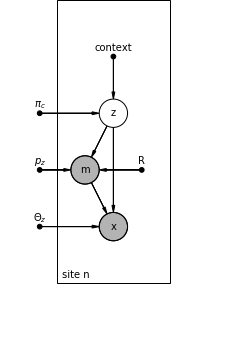
\includegraphics[width=0.3\textwidth]{pgm.png}
\caption{\label{fig:pgm} The probabilistic graphical model}
\end{figure}

What does the model know? What doesn't it know? 

%%%
\subsection{EM algorithm}
We may use the EM algorithm to estimate the hyperparameters $\vpi$ and $\vp$. We can then compute the posterior probability of the latent variable $z$ to determine whether a variant is an orientation artifact and thus should be filtered.

\subsubsection{E step}
In the E step, we compute the responsibility of the $k$th component of $z$, denoted $\gamma_{nk} = p(z_{nk} | x_n, m_n)$. $\gamma_{nk}$ is the posterior probability of $k$th component of $z$ given the observed variables $x_n$ and $m_n$. By Bayes rule we have

\begin{align}
\gamma^*_{nk} &\propto p(z_{k} | x_n) \nonumber \\
		        &\propto p(z_{k}) p(m_n | z_k, p_{z} ) p(x_n | m_n ) \nonumber \\
		        &= \pi_k  \{ p_{z}^{m_n} (1-p_k)^{R - m_n} \} \{ \theta_k^{x_n} (1 - \theta_k)^{m_n - x_n} \}
\end{align}

where $R$ is the number of reads at site $n$, and the asterisk over $\gamma^*_{nk}$ denotes that the responsibility is not normalized and thus is not a probability. We normalize each responsibility by dividing by their sum as below.

\begin{align}
\gamma_{nk} = \frac{\gamma^*_{nk}}{\sum_{k'} \gamma^*_{nk'}}
\end{align}

\subsubsection{M step}
In the M step, we compute the expectation of the complete-data log likelihood with respect to the posterior distribution over $z$ (so $\E$ stands for $\E_{Z \sim p(Z|X,M)}$). Thus,

\begin{align}
\E [ \ln p(X, M , Z | \vpi, \vp, \vtheta) ] &= \E [ \ln \prod_{n = 1}^{N}  p(Z) p(M | Z, p_{z} ) p(X | M, Z ) ] \nonumber \\
							&= \E [ \ln \prod_{n = 1}^{N} \{ \prod_{k = 1}^{K} \pi_k^{z_{kn}} \} \{ \prod_{k = 1}^{K} ( p_k^{m_n} (1-p_k)^{R - m_n} ) ^{z_{nk}} \} \{ \prod_{k = 1}^{K} ( \theta_k^{x_n} (1 - \theta_k)^{m_n - x_n} )^{z_{nk}} \} ] \notag \\
							&= \E [ \ln \prod_{n = 1}^{N} \prod_{k = 1}^{K} ( \pi_k  p_{k}^{m_n} (1-p_k)^{R - m_n} \theta_k^{x_n} (1 - \theta_k)^{m_n - x_n} )^{z_{nk}} ]  \nonumber \\
							&= \E [ \sum_{n = 1}^{N} \sum_{k = 1}^{K} z_{nk} \{ \ln \pi_k  + m_n \ln p_k + (R - m_n) \ln (1-p_k) + \notag \\
							&\phantom{---------------} x_n \ln \theta_k + (m_n - x_n) \ln (1 - \theta_k) \} ]  \nonumber \\
							&= \sum_{n = 1}^{N} \sum_{k = 1}^{K} \gamma_{nk} \{ \ln \pi_k  + m_n \ln p_k + (R - m_n) \ln (1-p_k) + \notag \\
						    &\phantom{---------------} x_n \ln \theta_k + (m_n - x_n) \ln (1 - \theta_k) \label{eq:expjointLL} \}
\end{align} 

where $K = |Z|$, $X$ is the design matrix whose $n$th row is $x_n$ ($M$ and $Z$ are defined analogously), and $\E [ z_{nk} ] = \gamma_{nk}$. We define the next three terms mainly for convenience but also because they have nice interpretations.

\begin{align}
N_k      &= \sum_n \gamma_{nk} \label{eq:nk} \\
\bar{x}_k  &= \frac{1}{N_k} \sum_n \gamma_{nk} x_n \label{eq:xbar} \\
\bar{m}_k &= \frac{1}{N_k} \sum_n \gamma_{nk} m_n \label{eq:mbar}
\end{align}

$N_k$ is the effective number of samples that were in state $z = z_k$, while $\bar{x}_k$ and $\bar{m}_k$ are the sample means of $x$ and $m$ weighted by each sample's responsibility in explaining the $k$th component. We now take the derivative of (\ref{eq:expjointLL}) with respect to $\theta_k, p_k, \pi_k$ and set each equal to 0, which yields:

\begin{align}
\frac{\partial}{\partial \theta_k} &= \sum_n \gamma_{nk} \Big( \frac{ x_n}{\theta_k} - \frac{m_n - x_n}{1- \theta_k} \Big)\\
					      &= \frac{N_k \bar{x}_k}{\theta_k} - \frac{N_k \bar{m}_k - N_k \bar{x}_k}{1- \theta_k} = 0
\end{align}

where we used (\ref{eq:xbar}) and (\ref{eq:mbar}). Solving for $\theta_k$, we get

\begin{align}
\hat{\theta}_k = \frac{\bar{x}_k}{\bar{m}_k} \label{eq:theta}
\end{align}

Derivative with respect to $p_k$ is completely analogous. In the end, we get

\begin{align}
\hat{p}_k = \frac{\bar{m}_k}{R} \label{eq:p}
\end{align}

Finally we take the derivative with respect to $\pi_k$ under the constraint $\sum_k \pi_k = 1$. Using a Lagrange multiplier to account for the constraint, we get

\begin{align}
\frac{\partial}{\partial \pi_k} \{ \E [ \ln p(X, M , Z | \vpi, \vp, \vtheta) ] + \lambda ( \sum_k \pi_k - 1)\} &= \sum_n \frac{\gamma_{nk}}{\pi_k} + \lambda \nonumber \\
																   &= \frac{N_k}{\pi_k} + \lambda = 0 \label{eq:dpi}
\end{align}

where $\lambda$ is the Lagrange multiplier. Rearranging (\ref{eq:dpi}) and summing over $k$, we get

\begin{align*}
\sum_k N_k &= \sum_k - \lambda \pi_k \\
      \lambda &= - N 
\end{align*}

Plugging in for $\lambda$ in (\ref{eq:dpi}) we obtain

\begin{equation}
\hat{\pi}_k = \frac{N_k}{N}
\end{equation}

% TODO: Discuss the forms of these update equations
% Initialize parameters, and iterate E and M-steps.



%%%%%%%%%%
\section{July 14th meeting with David}

When building a model, we'd like to know what information the model knows about. The previous model knew that 

\begin{itemize}
\item the probability of orientation bias depends on context
\item if orientation bias, most \underline{alt} reads have one or the other orientation
\end{itemize}

But the model did not know, crucially, that if there's orientation bias, there must be some alt reads. Since we were looking at sites that have alt reads, the model didn't know 

We then decided to add the variable $m$ to the model.  Once the model was updated, we went over different scenarios: what would happen if 
\begin{itemize}
\item $n = 100, m = 10, x = 5$ 
\item $n = 100, m = 1, x = 1$
\item $n = 100, m = 0, x = 0$
\end{itemize}

How does each part of the model vote, so to speak, for or against such data? The different components are $p(m|z), p(x|m), p(z | \pi)$. The first case rules 
When the later likelihoods don't favor one of the other, the final vote falls on $p(z | \pi)$ which, assuming we already have the hyperparameters learned over all sites, uses the prior across all sites to vote one way or another. That is, when data is not very informative, when it doesn't tell us one way or another, we use the prior knowledge to make the decision, which makes sense.

When mean field theory is used, the conjugacy across nodes is not crucial. Conjugacy between immediate neighbors makes life easier.

$m$ could be binomial. Or it could be beta-binomial. Beta-binomial has larger spread when $n$ is large or something. 

At one point I suggested that $m|z = \mathrm{no bias}$ be a mixture, between somatic variant (where $m$ can be large) or hom ref (where $m$). Instead I could just add more values to the $z$ variable such that $z \in \{ \text{F1R2}, \text{F2R1}, \text{Balanced Hom Ref}, \text{Balanced Somatic}, \text{Germline} \}$.




\end{document}